% Session 3: Verification Through to the Paper
% Structure and timings: admin/course_plan_4_sessions.md (blocks 23-29)
% Beamer Presentation — Claude Code for Academic Researchers
\documentclass[aspectratio=169, 11pt]{beamer}

% ── Theme and Colors ──────────────────────────────────────────────
\usetheme{Madrid}
\usecolortheme{default}

% Custom colors
\definecolor{anthropic}{RGB}{50, 50, 80}
\definecolor{accent}{RGB}{180, 90, 40}
\definecolor{lightgray}{RGB}{245, 245, 245}

\setbeamercolor{structure}{fg=anthropic}
\setbeamercolor{frametitle}{bg=anthropic, fg=white}
\setbeamercolor{title}{bg=anthropic, fg=white}
\setbeamercolor{block title}{bg=anthropic, fg=white}
\setbeamercolor{block body}{bg=lightgray}
\setbeamercolor{alerted text}{fg=accent}

\setbeamerfont{title}{size=\Large, series=\bfseries}
\setbeamerfont{frametitle}{size=\large, series=\bfseries}

% ── Packages ──────────────────────────────────────────────────────
\usepackage{graphicx}
\usepackage{booktabs}
\usepackage{array}
\newcolumntype{L}[1]{>{\raggedright\arraybackslash}p{#1}}
\usepackage{listings}
\usepackage{fontenc}
\usepackage{hyperref}
\usepackage{appendixnumberbeamer} % footer page count stops at \appendix
\usepackage{tikz}
\usetikzlibrary{positioning}

\lstset{
  basicstyle=\ttfamily\small,
  backgroundcolor=\color{lightgray},
  frame=single,
  framerule=0pt,
  breaklines=true,
  columns=fullflexible,
  literate={_}{\_}1,
}

% ── Metadata ──────────────────────────────────────────────────────
\title{Session 3: Verification Through to the Paper}
\subtitle{Estimation, Robustness, \LaTeX{}, Git, and Results to Paper}
\author{Brady Allardice}
\date{}
\institute{UPF \& IBEI}

% ══════════════════════════════════════════════════════════════════
\begin{document}

\begin{frame}[plain]
  \titlepage
\end{frame}

% ══════════════════════════════════════════════════════════════════
%  OPENING, RITUAL, CHECK-IN  [0:00-0:05]
% ══════════════════════════════════════════════════════════════════

\begin{frame}{Where We Are}
  \textbf{Session 1:} What Claude Code is and how it works.

  \vspace{0.5em}
  \textbf{Session 2:} Staying in control: context, plan mode, and verification. You merged the Swiss franc data with a builder tab and an independent checker tab.

  \vspace{0.5em}
  \textbf{Session 3:} From a verified dataset to a paper.

  \vspace{0.8em}
  Today you will:
  \begin{enumerate}
    \item Finish the Swiss franc project: estimate, account for every observation, run robustness checks, produce a \LaTeX{} table
    \item Set up \LaTeX{} in VS Code and learn git as the undo button for agent edits
    \item Put results into a paper, have Claude Code write the text, and check every number against the table
  \end{enumerate}

  \vspace{0.5em}
  \alert{A number in a paper is a claim. Today you check it before it leaves the project.}
\end{frame}

\begin{frame}[fragile,label=ritual]{Start-of-Session Ritual}
  Work on a copy, not inside the shared repo. Do this now:

  \vspace{0.2em}
  \begin{columns}[t]
    \column{0.48\textwidth}
    \textbf{Mac / Linux}
    \begin{lstlisting}[basicstyle=\ttfamily\tiny]
# Already cloned? Update:
cd ~/claude-code-workshop && git pull

# First time:
git clone https://github.com/
  bradyallardice/claude-code-workshop.git

# Copy and open
cp -r session_3/ ~/my_workspace/session_3/
cd ~/my_workspace/session_3
code .
    \end{lstlisting}

    \column{0.48\textwidth}
    \textbf{Windows (PowerShell)}
    \begin{lstlisting}[basicstyle=\ttfamily\tiny]
# Already cloned? Update:
cd ~\claude-code-workshop; git pull

# First time:
git clone https://github.com/
  bradyallardice/claude-code-workshop.git

# Copy and open
Copy-Item -Recurse session_3 `
  ~\my_workspace\session_3
cd ~\my_workspace\session_3
code .
    \end{lstlisting}
  \end{columns}

  \vspace{0.2em}
  {\small \textbf{Then reopen your \texttt{session\_2} copy} in a new VS Code window (File $\rightarrow$ New Window $\rightarrow$ Open Folder). Part 2 continues in it.} \hfill \hyperlink{gitpull}{\beamergotobutton{git pull fails?}}
\end{frame}

\begin{frame}{Check-In: Claude Code in Your Work}
  \textbf{Since Session 2, have you tried Claude Code on your own research?}

  \vspace{0.5em}
  \begin{itemize}
    \item \textbf{What for:} what kind of tasks?
    \item \textbf{Pain points:} what was frustrating or hard?
    \item \textbf{Trust:} are you confident in the code it produces?
    \item \textbf{Decisions:} did it make a choice you did not ask for? Did you notice at the time?
  \end{itemize}
\end{frame}

% ══════════════════════════════════════════════════════════════════
%  BLOCK 23: VERIFICATION EXTRAS  [0:05-0:10]
% ══════════════════════════════════════════════════════════════════

\begin{frame}{The Requirements-to-Tests Matrix}
  \footnotesize
  \renewcommand{\arraystretch}{1.2}
  \begin{tabular}{@{}L{0.27\textwidth}L{0.21\textwidth}L{0.42\textwidth}@{}}
    \toprule
    \textbf{Requirement} & \textbf{Test} & \textbf{Passing condition} \\
    \midrule
    Merge keeps every respondent & Row-count and key test & 2,044 rows; \texttt{respondent\_id} unique \\
    Outcome built as defined & Variable-construction test & \texttt{supports\_intervention} is 1 exactly for ``some'' or ``big'' \\
    Control is the reference arm & Specification test & The omitted category is \texttt{cntrl} \\
    Survey weights are used & Independent recomputation & Logistic of the base-model intercept equals the weighted control share from the raw CSV \\
    N is explained for every model & Sample accounting & Rows in $-$ rows dropped (by reason) = N used \\
    Every specification is reported & Output manifest & All specifications are in the table, each with its N \\
    \bottomrule
  \end{tabular}

  \vspace{0.5em}
  \small
  \alert{Write the matrix before the code.} A requirement with no test is unverified.
\end{frame}

\begin{frame}[fragile]{The Audit Report: Evidence, Not ``All Tests Passed''}
  \begin{lstlisting}[basicstyle=\ttfamily\footnotesize]
## Audit report
Tests run:         commands; passed / failed / skipped
Requirements:      each requirement -> its test
Not tested:        anything without a test, and why
Numerical checks:  our value vs. independent value
Needs your call:   choices Claude proposed
Not covered:       identification, construct validity
  \end{lstlisting}

  \vspace{0.3em}
  \begin{block}{What the report is for}
    Not for Claude Code to declare the research correct. It documents what was exercised, against which expectation, and what remains uncertain.
  \end{block}
\end{frame}

\begin{frame}{Two More Safeguards}
  \begin{columns}[T]
    \begin{column}{0.48\textwidth}
      \textbf{Replicate before you extend}
      \begin{enumerate}
        \small
        \item Give Claude Code the original code or description
        \item Ask it to replicate a key table
        \item Compare with the published result
        \item Only then begin your extension
      \end{enumerate}
      {\small If you cannot reproduce the baseline, nothing built on it is interpretable.}
    \end{column}
    \begin{column}{0.48\textwidth}
      \textbf{Use a second agent as a critic}
      \begin{enumerate}
        \small
        \item Agent 1 writes the code
        \item Open a new conversation (Agent 2) and ask: ``Read the analysis script and identify any bugs, silent data loss, or decisions that could change the results.''
      \end{enumerate}
      {\small This is a critic: it reads the code. Session 2's checker was stricter, because it never saw the code at all and worked from the codebook.}
    \end{column}
  \end{columns}

  \vspace{0.8em}
  \alert{Treat your agents like co-authors who check each other's work, not a single assistant you trust unconditionally.}
\end{frame}

\begin{frame}{What to Delegate, What to Verify, What to Keep}
  \begin{columns}[T]
    \begin{column}{0.32\textwidth}
      {\color{green!50!black}\textbf{Delegate freely}}\\[0.3em]
      {\small
      Boilerplate \& docs\\
      File management\textsuperscript{\dag}\\
      Reformatting code}
    \end{column}
    \begin{column}{0.32\textwidth}
      {\color{accent}\textbf{Delegate + verify}}\\[0.3em]
      {\small
      Data loading \& cleaning\\
      Data merges\\
      Variable construction\\
      Summary statistics\\
      Robustness variants\\
      Visualization\\
      \LaTeX{} tables}
    \end{column}
    \begin{column}{0.32\textwidth}
      {\color{red!70!black}\textbf{Do not delegate}}\\[0.3em]
      {\small
      Choosing specifications\\
      Interpreting results\\
      Identification strategy\\
      Sample selection\\
      Causal claims}
    \end{column}
  \end{columns}

  \vspace{0.5em}
  {\scriptsize \textsuperscript{\dag} Be careful with file management --- Claude Code can delete files. Always review before approving.}

  \vspace{0.5em}
  The test: \textit{If a referee questioned this choice, who would need to answer --- you or the RA?}

  \vspace{0.5em}
  Today's exercise focuses on the middle column: tasks where Claude Code is productive but where you must verify every output.
\end{frame}

% ══════════════════════════════════════════════════════════════════
%  BLOCK 24: EXERCISE PART 2  [0:10-0:35]
% ══════════════════════════════════════════════════════════════════

\begin{frame}{Before You Start: Reopen Your Session 2 Folder}
  Part 2 continues the project you started in Session 2. Open \texttt{my\_workspace/session\_2} in a \textbf{new VS Code window}.

  \vspace{0.5em}
  \textbf{Check that these exist:}
  \begin{itemize}
    \item \texttt{CLAUDE.md} with the verification protocol
    \item Your merge script and \texttt{output/merged\_survey.csv}
    \item Your merge tests, and they pass
  \end{itemize}

  \vspace{0.5em}
  \textbf{If your merge did not finish:} ask Claude Code to finish it and run its tests first. Do not estimate on a merge you have not checked. Give this at most five minutes.

  \vspace{0.5em}
  \alert{Start a new conversation. The old one carries Session 2's context.}
\end{frame}

\begin{frame}{Exercise Part 2: Specify and Estimate (25 min)}
  \begin{enumerate}
    \setcounter{enumi}{3}
    \item \textbf{Base model:} Logistic regression of \texttt{supports\_intervention} on \texttt{treatment}.
    \begin{itemize}
      \small
      \item Use survey weights. What should the reference category be? Tell Claude Code explicitly.
      \item \alert{Independent check:} the logistic of the intercept should equal the weighted control-group share, computed straight from the raw CSV
    \end{itemize}

    \vspace{0.2em}
    \item \textbf{Add FX exposure.} Did the sample size change? Why or why not?

    \vspace{0.2em}
    \item \textbf{Add demographic controls:} age, female, education, urban/rural, income, left-right.
    \begin{itemize}
      \small
      \item \alert{Before running: predict how many observations you will have.} Then check.
    \end{itemize}

    \vspace{0.2em}
    \item \textbf{Add an interaction} between treatment and FX exposure.
  \end{enumerate}

  \vspace{0.4em}
  {\small \alert{For every model, reconcile N:} rows in $-$ rows dropped (by reason) = N used.}
\end{frame}

\begin{frame}{Part 2 Debrief: What Happened to Your Sample?}
  \textbf{How many observations did you have in each model?}

  \vspace{1em}
  \pause
  \begin{alertblock}{The Missing Data Trap}
    Adding control variables can silently change your sample.
  \end{alertblock}

  \vspace{0.3em}
  \begin{tabular}{lrl}
    \toprule
    \textbf{Specification} & \textbf{N} & \textbf{What happened} \\
    \midrule
    Treatment only & 2,036 & Full sample (8 missing outcome) \\
    + FX exposure & 2,035 & 1 more dropped (missing FX status) \\
    + age, female, education, urban/rural & 2,035 & No additional missingness \\
    + income quintile & 1,473 & \color{red!70!black}{562 missing income} \\
    + left-right scale (without income) & 1,499 & \color{red!70!black}{536 missing left-right} \\
    + both & 1,151 & \color{red!70!black}{884 dropped: 43\% of the sample} \\
    \bottomrule
  \end{tabular}

  \vspace{0.5em}
  \textbf{Did Claude Code mention this when it added the controls?}
\end{frame}

% ══════════════════════════════════════════════════════════════════
%  BLOCK 25: ROBUSTNESS WORKFLOW AND EXERCISE PART 3  [0:35-1:00]
% ══════════════════════════════════════════════════════════════════

\begin{frame}{The Robustness Workflow}
  \centering
  {\large You specify the core analysis.\\
  Claude Code generates the variations.\\
  You verify each one.}

  \vspace{1.5em}
  \textbf{Claude Code never chooses what robustness checks to run.}

  \vspace{1em}
  \textbf{For each specification, check:}
  \begin{itemize}
    \item Does it use the right sample? (What is N?)
    \item Does the code match what you asked for?
    \item Are the coefficients in a plausible range?
    \item Do the signs on control variables make sense?
  \end{itemize}

\end{frame}

\begin{frame}{Exercise Part 3: Robustness and Output (25 min)}
  \begin{enumerate}
    \setcounter{enumi}{7}
    \item \textbf{Generate robustness checks} from your base model:
    \begin{itemize}
      \item With and without survey weights
      \item Different control sets (track how N changes each time!)
      \item Collapse three treatment arms into ``any information'' vs.\ control
      \item Restrict to complete cases so N is constant across specs
    \end{itemize}

    \vspace{0.3em}
    \item \textbf{Format as \LaTeX.} Produce a publication-style regression table with all specifications side by side, and compile to PDF.
    \begin{itemize}
      \small
      \item Output manifest test: every specification appears in the table, each with its N
    \end{itemize}

    \vspace{0.3em}
    \item \textbf{Audit report.} Ask Claude Code for \texttt{output/audit\_report.md}, in the format from the audit-report slide.

    \vspace{0.3em}
    \item \textbf{Commit.} Save all scripts, tests, output, and the \LaTeX{} table.
  \end{enumerate}
\end{frame}

\begin{frame}{What to Watch For During the Exercise}
  This exercise is designed to surface moments where Claude Code makes choices for you.

  \vspace{0.5em}
  \begin{itemize}
    \small
    \item \textbf{Reference categories:} Did it set treatment to ``control'' or pick alphabetically?
    \item \textbf{Missing data:} When you added controls, how many observations did you lose? Did Claude Code mention this?
    \item \textbf{Survey weights:} Did it use them unless you told it to?
    \item \textbf{Income = 0:} ``No income'' is coded as 0. How did Claude Code treat it?
    \item \textbf{Tests:} Did it copy the pipeline's own output in as an expected value, or edit one to get a pass?
  \end{itemize}

  \vspace{0.8em}
  \alert{These are the moments where your judgment matters.}\\
  The workflow is: notice the decision, direct Claude Code explicitly, then verify the output.
\end{frame}

\begin{frame}{Debrief}
  \textbf{Discussion questions:}

  \vspace{0.5em}
  \begin{enumerate}
    \small
    \item How many observations did you lose when you added controls? Did Claude Code tell you?
    \item How many of your robustness specifications were correct on the first try?
    \item What did you catch in the plan that you would have missed in the output?
    \item Did any test fail? Did Claude Code fix the code, or change the test?
  \end{enumerate}

  \vspace{0.5em}
  \begin{block}{Key takeaway}
    The tests, the assertions, and the plan review are not extra work --- they are the workflow. The 30 seconds it takes to read a plan or check a sample size can save hours of debugging downstream.
  \end{block}
\end{frame}

% ══════════════════════════════════════════════════════════════════
%  BLOCK 26: LATEX IN VS CODE, GIT AS THE UNDO BUTTON, OVERLEAF BRIDGE  [1:00-1:22]
% ══════════════════════════════════════════════════════════════════

\begin{frame}{\LaTeX{} Tables: Bringing Results Into Your Paper}
  Until now, your results are printed to the console or saved as CSVs.\\
  In your actual workflow, they need to end up in a paper.

  \vspace{0.8em}
  \textbf{Why this matters:}
  \begin{itemize}
    \item Claude Code can write \LaTeX{} tables directly from regression output
    \item The table lives in your project directory, under version control
    \item When you update the analysis, Claude Code updates the table
    \item No manual reformatting, no copy-paste errors
  \end{itemize}

  \vspace{0.8em}
  \textbf{Next:} the paper that table goes into. We bring it into VS Code, next to the code and data.

  \vspace{0.5em}
  \begin{block}{The bigger idea}
    The more of your research that lives inside the project directory, the more Claude Code
    can operate on. Code, data, output, tables --- and eventually the paper itself.
  \end{block}
\end{frame}

\begin{frame}{The Problem with Overleaf}
  \textbf{Most researchers keep their paper in a separate tool.}

  \vspace{0.5em}
  \begin{itemize}
    \item Code lives in a project directory (or on your Desktop)
    \item Data lives next to the code (maybe)
    \item The paper lives in Overleaf (or Word, or Google Docs)
  \end{itemize}

  \vspace{0.8em}
  \textbf{What this means for Claude Code:}
  \begin{itemize}
    \item It cannot read your paper
    \item It cannot check the methods section against your code
    \item It cannot update a table when the analysis changes
    \item It cannot commit changes to your paper alongside code changes
  \end{itemize}

  \vspace{0.8em}
  \begin{alertblock}{The Limitation}
    If Claude Code cannot see it, Claude Code cannot operate on it.\\
    Your paper is the biggest piece of your project that is currently invisible.
  \end{alertblock}
\end{frame}

\begin{frame}{The Solution: \LaTeX{} in VS Code}
  \textbf{Bring your paper into the project directory.}

  \vspace{0.8em}
  \begin{itemize}
    \item Your \texttt{.tex} file lives alongside \texttt{scripts/} and \texttt{data/}
    \item Claude Code can read it, write it, and edit it --- just like any other file
    \item Changes to the paper are tracked by git, just like code changes
    \item Coauthors review changes through version control, not ``track changes''
  \end{itemize}

  \vspace{0.8em}
  \textbf{What becomes possible:}
  \begin{itemize}
    \item Claude Code writes a methods section and you verify it against the code
    \item The analysis changes $\rightarrow$ the table updates $\rightarrow$ the paper updates
    \item Every version of the paper is recoverable through git
  \end{itemize}

  \vspace{0.5em}
  \begin{block}{The Point}
    This is not about \LaTeX{} vs.\ Word. It is about bringing your paper into the agentic workflow.
  \end{block}
\end{frame}

\begin{frame}{\LaTeX{} in VS Code: The Setup}
  \textbf{What you need (should be installed from pre-work):}
  \begin{enumerate}
    \item A \TeX{} distribution: TeX Live (Linux/Windows) or MacTeX (Mac)
    \item The \textbf{LaTeX Workshop} extension in VS Code
  \end{enumerate}

  \vspace{0.8em}
  \textbf{What you get:}
  \begin{itemize}
    \item Syntax highlighting for \texttt{.tex} files
    \item One-click compilation to PDF
    \item PDF preview in a split pane --- side by side with your code
    \item Error messages in the VS Code terminal
  \end{itemize}

  \vspace{0.8em}
  \textbf{The workflow:}\\
  Edit \texttt{.tex} $\rightarrow$ Save $\rightarrow$ Auto-compile $\rightarrow$ PDF updates in the preview pane.

  \vspace{0.5em}
  You never leave VS Code. Your paper is right next to your code.

  \vspace{0.3em}
  \hfill \hyperlink{latexbasics}{\beamergotobutton{New to \LaTeX{}?}}
\end{frame}

\begin{frame}[fragile]{\LaTeX{} Workshop: Essential Commands}
  \textbf{Three ways to compile:}

  \vspace{0.3em}
  \begin{columns}[T]
    \column{0.5\textwidth}
    \textbf{Keyboard Shortcuts (Mac):}
    \begin{lstlisting}[basicstyle=\ttfamily\tiny]
Cmd+Alt+B   Compile to PDF
Cmd+Alt+V   Open PDF preview
    \end{lstlisting}

    \textbf{Keyboard Shortcuts (Windows/Linux):}
    \begin{lstlisting}[basicstyle=\ttfamily\tiny]
Ctrl+Alt+B  Compile to PDF
Ctrl+Alt+V  Open PDF preview
    \end{lstlisting}

    \column{0.5\textwidth}
    \textbf{Or click the green button:}\\
    \vspace{0.3em}
    
\includegraphics[width=0.15\textwidth]{img/compile_button.png}
  \end{columns}

  \vspace{0.8em}
  \textbf{Once the preview is open:}
  \begin{itemize}
    \item Right-click the PDF preview tab and select \texttt{Move into Side Panel}
    \item Now you have code on the left, PDF on the right
  \end{itemize}

  \vspace{0.3em}
  \textbf{Optional: Auto-compile on save}\\
  Add to VS Code settings: \texttt{"latex-workshop.latex.autoBuild.run": "onFileChange"}
\end{frame}

\begin{frame}{\LaTeX{} Errors and the Problems Pane}
  When you compile, LaTeX Workshop checks for errors and syntax issues. They appear in the \textbf{Problems} pane at the bottom of VS Code.

  \vspace{0.5em}
  \textbf{To view the Problems pane:}
  \begin{itemize}
    \item Keyboard: \texttt{Ctrl+Shift+M} (or \texttt{Cmd+Shift+M} on Mac)
    \item Menu: \texttt{View} \textrightarrow{} \texttt{Problems}
  \end{itemize}

  \vspace{0.8em}
  \centering
  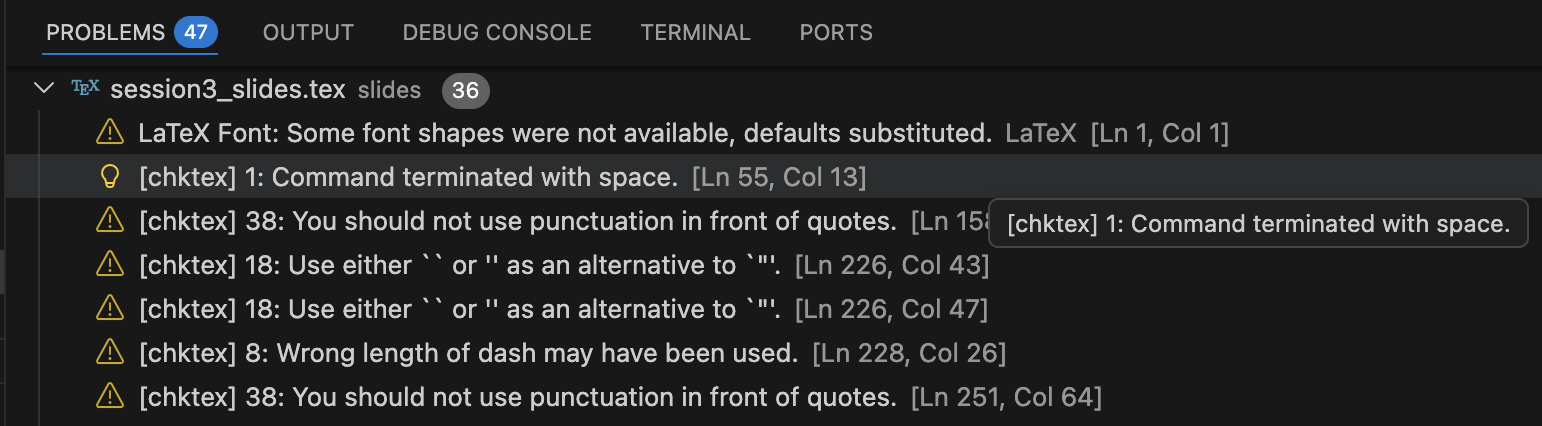
\includegraphics[width=0.8\textwidth]{img/problems_latex.png}

  \vspace{0.3em}
  {\small Errors and warnings appear here with line numbers. Click any error to jump to that line in your \texttt{.tex} file.}
\end{frame}

\begin{frame}{Why All This Matters for Claude Code}
  \textbf{The payoff:} Everything is in one place. Your code, your data, your \LaTeX{} document, and your compilation errors are all visible to Claude Code.

  \vspace{0.8em}
  \textbf{Claude Code can:}
  \begin{itemize}
    \item \textbf{See the error:} Claude Code reads the Problems pane and helps you fix it
    \item \textbf{Write the \LaTeX:} Describe what you want (a table, a figure reference, a citation) and Claude Code writes it
    \item \textbf{Check consistency:} Ask Claude Code to verify that your methods section matches your actual code
    \item \textbf{Iterate quickly:} Write → Compile → Show error to Claude Code → Revise → Repeat
  \end{itemize}

  \vspace{0.8em}
  \begin{block}{The Workflow}
    Your \texttt{.tex} file is no longer separate from your research. It is part of your project, subject to the same verification and version control as your code.
  \end{block}
\end{frame}

\begin{frame}{Why Git Matters for Agentic Coding}
  \textbf{The problem:} Claude Code modifies your files directly.

  \vspace{0.5em}
  \begin{itemize}
    \item It might change a file you did not ask it to change
    \item It might overwrite working code with something broken
    \item It might make 10 changes when you only wanted 3
  \end{itemize}

  \vspace{0.8em}
  \textbf{Without git:} You try to manually undo changes. You are not sure what the file looked like before. You lose work.

  \vspace{0.5em}
  \textbf{With git:} You see exactly what changed, line by line. You revert anything you do not want. You never lose work.

  \vspace{0.8em}
  \begin{alertblock}{The Rule}
    Never let Claude Code touch your project without a recent commit to fall back on.
  \end{alertblock}
\end{frame}

\begin{frame}[fragile]{The Minimum Viable Git Workflow}
  \begin{center}
  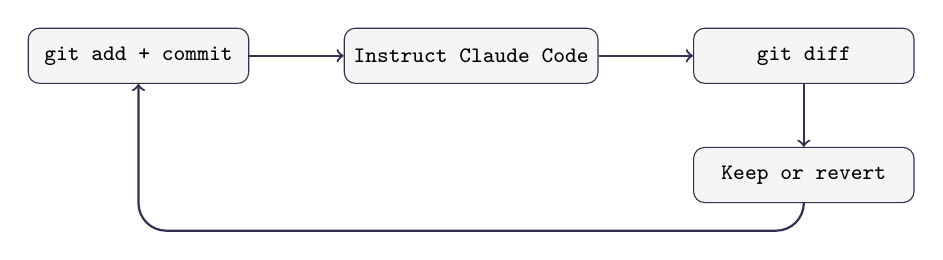
\begin{tikzpicture}[
    node distance=0.8cm and 1.2cm,
    box/.style={draw=anthropic, fill=lightgray, rounded corners, minimum width=2.8cm, minimum height=0.7cm, align=center, font=\footnotesize\ttfamily},
    arr/.style={->, thick, color=anthropic}
  ]
    \node[box] (commit) {git add + commit};
    \node[box, right=of commit] (instruct) {Instruct Claude Code};
    \node[box, right=of instruct] (diff) {git diff};
    \node[box, below=of diff] (decide) {Keep or revert};

    \draw[arr] (commit) -- (instruct);
    \draw[arr] (instruct) -- (diff);
    \draw[arr] (diff) -- (decide);
    \draw[arr, rounded corners=10pt] (decide.south) -- ++(0,-0.35) -| (commit.south);
  \end{tikzpicture}
  \end{center}

  {\small
  \begin{tabular}{ll}
    \toprule
    \textbf{Command} & \textbf{What it does} \\
    \midrule
    \texttt{git add -A \&\& git commit -m "msg"} & Snapshot your current state \\
    \texttt{git diff} & See what changed since last commit \\
    \texttt{git checkout -- file.py} & Undo changes to a specific file \\
    \texttt{git log --oneline} & See your commit history \\
    \bottomrule
  \end{tabular}
  }
\end{frame}

\begin{frame}[fragile]{Command 1: \texttt{git init}}
  \textbf{What it does:} Turns a regular folder into a git project.

  \vspace{0.5em}
  \begin{lstlisting}
git init
  \end{lstlisting}

  \vspace{0.5em}
  \begin{itemize}
    \item You run this \textbf{once}, when you start a new project
    \item It creates a hidden \texttt{.git/} folder that stores your project's history
    \item Nothing else changes --- your files stay exactly as they are
  \end{itemize}

  \vspace{0.8em}
  Think of it as saying: ``I want to start tracking this folder.''

  \vspace{0.5em}
  \begin{block}{Note}
    Your session folders are copies without a \texttt{.git} folder, so each project needs its own \texttt{git init}. \texttt{git status} tells you whether a folder is already tracked.
  \end{block}
\end{frame}

\begin{frame}[fragile]{Command 2: \texttt{git add}}
  \textbf{What it does:} Selects which files to include in your next save point.

  \vspace{0.5em}
  \begin{lstlisting}
git add -A
  \end{lstlisting}

  \vspace{0.5em}
  \begin{itemize}
    \item \texttt{-A} means ``add everything that changed'' --- new files, modified files, deleted files
    \item This does not save anything yet. It just marks what will be included in the next commit.
  \end{itemize}

  \vspace{0.8em}
  You can also add specific files instead of everything:
  \begin{lstlisting}
git add scripts/analysis.py
  \end{lstlisting}

  \vspace{0.5em}
  Think of it as putting files in a box before sealing it. \texttt{git add} fills the box; \texttt{git commit} seals it.
\end{frame}

\begin{frame}[fragile]{Command 3: \texttt{git commit}}
  \textbf{What it does:} Saves a snapshot of everything you added.

  \vspace{0.5em}
  \begin{lstlisting}
git commit -m "Clean merge script, verified row counts"
  \end{lstlisting}

  \vspace{0.5em}
  \begin{itemize}
    \item \texttt{-m} stands for ``message'' --- a short note describing what this snapshot contains
    \item The message goes in quotes. Write something your future self will understand.
    \item After committing, you have a permanent save point you can always return to.
  \end{itemize}

  \vspace{0.5em}
  \textbf{In practice, you can always run add and commit together (but you don't have to):}
  \begin{lstlisting}
git add -A && git commit -m "your message"
  \end{lstlisting}

  \vspace{0.3em}
  The \texttt{\&\&} just means ``run the second command after the first one finishes.''
\end{frame}

\begin{frame}[fragile]{Command 4: \texttt{git diff}}
  \textbf{What it does:} Shows you exactly what changed since your last commit.

  \vspace{0.5em}
  \begin{lstlisting}
git diff
  \end{lstlisting}

  \vspace{0.5em}
  The output looks like the diff view you already know from VS Code:
  \begin{itemize}
    \item Lines starting with \texttt{+} were added (green in VS Code)
    \item Lines starting with \texttt{-} were removed (red in VS Code)
    \item Everything else is unchanged context
  \end{itemize}

  \vspace{0.5em}
  \textbf{When to use it:} After Claude Code makes changes, run \texttt{git diff} to see \textit{everything} it touched --- not just the file it told you about.

  \vspace{0.5em}
  \begin{block}{Tip}
    You can also ask Claude Code: ``Run git diff and explain each change you made.''
  \end{block}
\end{frame}

\begin{frame}[fragile]{Command 5: \texttt{git log}}
  \textbf{What it does:} Shows you the history of all your commits.

  \vspace{0.5em}
  \begin{lstlisting}
git log --oneline
  \end{lstlisting}

  \vspace{0.5em}
  \textbf{Output looks like:}
  \begin{lstlisting}
a3f7b21 Add robustness checks
e5c9d04 Clean merge script, verified row counts
b1a2c33 Initial commit
  \end{lstlisting}

  \vspace{0.5em}
  \begin{itemize}
    \item Each line is one commit --- one save point
    \item The letters and numbers on the left are the commit ID
    \item The message on the right is what you wrote with \texttt{-m}
    \item Most recent commits are at the top
  \end{itemize}

  \vspace{0.3em}
  This is your project's timeline. You can always see what you did and when.
\end{frame}

\begin{frame}[fragile]{Command 6: \texttt{git checkout}}
  \textbf{What it does:} Undoes changes by restoring files to a previous committed state.

  \vspace{0.5em}
  \textbf{Undo uncommitted changes to one file:}
  \begin{lstlisting}
git checkout -- scripts/analysis.py
  \end{lstlisting}

  \vspace{0.4em}
  \textbf{Undo all uncommitted changes:}
  \begin{lstlisting}
git checkout -- .
  \end{lstlisting}

  \vspace{0.4em}
  \textbf{Go back several commits (rewind the whole project):}
  \begin{lstlisting}
git log --oneline         # find the commit you want
git checkout <commit-hash>  # jump to that commit
git checkout main         # come back to the latest
  \end{lstlisting}

  \vspace{0.3em}
  Or use \texttt{HEAD\~{}N} to go back \texttt{N} commits from your current position:
  \begin{lstlisting}
git checkout HEAD~3    # go back 3 commits
  \end{lstlisting}
\end{frame}

\begin{frame}[fragile]{\texttt{git checkout}: Your Undo Button}
  \textbf{The mental model:}
  \begin{itemize}
    \item \texttt{git checkout -- .} \quad\textrightarrow\ undo \textit{uncommitted} work
    \item \texttt{git checkout <hash>} \quad\textrightarrow\ travel back to any previous commit
    \item \texttt{git checkout main} \quad\textrightarrow\ return to the latest state
  \end{itemize}

  \vspace{0.8em}
  \textbf{Recovering if something goes wrong:}
  \begin{lstlisting}
git reflog    # shows every action you've taken
  \end{lstlisting}
  Even changes you thought were gone are usually recoverable.

  \vspace{0.5em}
  \begin{alertblock}{This all only works if you committed first}
    Checkout lets you jump between snapshots --- but you need snapshots to jump to. That is why you always commit before instructing Claude Code.
  \end{alertblock}
\end{frame}

\begin{frame}{Putting It Together: The Cycle}
  \textbf{Before every interaction with Claude Code:}

  \vspace{0.3em}
  \begin{enumerate}
    \item \texttt{git add -A \&\& git commit -m "message"} --- save your current state
    \item Give Claude Code an instruction
    \item \texttt{git diff} --- see what it changed
    \item Decide:
    \begin{itemize}
      \item Happy? $\rightarrow$ \texttt{git add -A \&\& git commit -m "message"}
      \item Not happy? $\rightarrow$ \texttt{git checkout -- .}
    \end{itemize}
    \item Repeat
  \end{enumerate}

  \vspace{0.5em}
  \begin{block}{The Mindset Shift}
    Commits are not milestones. They are save points --- like pressing Ctrl+S. Commit early, commit often, commit before every interaction with Claude Code.
  \end{block}

  \vspace{0.5em}
  
\end{frame}

\begin{frame}[fragile]{\texttt{.gitignore}: Telling Git What to Skip}
  A \texttt{.gitignore} file lists patterns for files git should never track. Place it in the folder where you ran \texttt{git init}.

  \vspace{0.08em}
  \textbf{Paths are relative to that folder.} Example:
  \begin{lstlisting}[basicstyle=\ttfamily\tiny]
my_project/              <- run "git init" here
  .gitignore            <- goes here
  code/
    analysis.py
  data/                 <- put in .gitignore
    raw/
    processed/
  output/               <- put in .gitignore
  \end{lstlisting}

  \vspace{0.08em}
  \textbf{Always include in .gitignore:}
  \begin{lstlisting}[basicstyle=\ttfamily\tiny]
.DS_Store
.env      <- usually contains sensitive information
*.pyc
__pycache__/
*.aux
*.log
  \end{lstlisting}

  \vspace{0.05em}
  Then add: \texttt{data/raw/}, \texttt{*.csv.gz}, any large files.
\end{frame}

\begin{frame}[fragile]{Git and Data: What Not to Track}
  Git is designed for \textbf{code and text files} --- things that change line by line.\\
  It is \textit{not} designed for large data files.

  \vspace{0.3em}
  \begin{columns}[T]
    \begin{column}{0.48\textwidth}
      \textbf{Commit:}
      \begin{itemize}
        \item Scripts (\texttt{.py}, \texttt{.R}, \texttt{.do})
        \item \LaTeX{} files (\texttt{.tex}, \texttt{.bib})
        \item Documentation (\texttt{CLAUDE.md})
        \item Small data files (under a few MB)
      \end{itemize}
    \end{column}
    \begin{column}{0.48\textwidth}
      \textbf{Do not commit:}
      \begin{itemize}
        \item Large datasets (50MB+)
        \item Output you can regenerate
        \item Sensitive data (PII, API keys)
      \end{itemize}
    \end{column}
  \end{columns}

  \vspace{0.5em}
  \begin{block}{Rule of Thumb}
    Commit what a collaborator needs to \textit{understand} your project. Skip what they could \textit{regenerate} by running the code.
  \end{block}
\end{frame}

\begin{frame}{If Your Coauthors Are on Overleaf}
  Moving your paper into VS Code does not mean abandoning your coauthors.

  \vspace{0.8em}
  \textbf{Overleaf supports git sync.} Overleaf itself acts as the git remote, so you push and pull like any other repository. No GitHub account is involved.

  \vspace{0.8em}
  \textbf{The setup:}
  \begin{enumerate}
    \item Enable git sync on your Overleaf project (requires a paid plan)
    \item Clone the Overleaf remote to your local machine
    \item Open the \texttt{.tex} files in VS Code and work with Claude Code as normal
    \item Push your changes back to Overleaf when ready; coauthors see them immediately
  \end{enumerate}

  \vspace{0.8em}
  \begin{block}{Result}
    You get Claude Code and version control. Your coauthors get Overleaf.\\
    Nobody has to change their entire workflow at once.
  \end{block}
\end{frame}

\begin{frame}{The Hybrid Workflow}
  \textbf{You (VS Code + Claude Code):}
  \begin{itemize}
    \item Edit \texttt{.tex} locally, ask Claude Code to update tables, fix references, rewrite paragraphs
    \item Commit changes to git --- every edit is tracked and reversible
    \item Push to Overleaf when a section is ready for coauthor review
  \end{itemize}

  \vspace{0.8em}
  \textbf{Your coauthors (Overleaf):}
  \begin{itemize}
    \item Review and comment in the Overleaf interface as usual
    \item Make edits directly in Overleaf
    \item Their changes are commits you can pull locally
  \end{itemize}

  \vspace{0.8em}
  \textbf{Caveat:} merge conflicts are possible if you and a coauthor edit the same lines simultaneously --- the same risk as any shared git repo. Pull before you push.
  \vfill
  \hyperlink{backmatter}{\beamerreturnbutton{Back matter}}
\end{frame}

% ══════════════════════════════════════════════════════════════════
%  BLOCK 27: LIVE DEMO, THE FULL LOOP  [1:22-1:30]
% ══════════════════════════════════════════════════════════════════

\begin{frame}{Live Demo: Building a Paper from Scratch}
  \textbf{What I'm going to show you:}

  \vspace{0.5em}
  I have a folder with pre-generated outputs from a fake analysis of \textit{this course}:
  \begin{itemize}
    \item Summary statistics table (\texttt{.tex})
    \item Regression results table (\texttt{.tex})
    \item Four figures: enrollment, satisfaction, attrition, earnings effect
  \end{itemize}

  \vspace{0.5em}
  \textbf{Starting from nothing,} I'll use Claude Code to:
  \begin{enumerate}
    \item Create a blank \texttt{course\_paper.tex} file
    \item Write methods and data sections describing the study
    \item Pull in the pre-generated tables with \texttt{\textbackslash input\{...\}}
    \item Embed the figures with \texttt{\textbackslash includegraphics\{...\}}
    \item Compile to PDF and fix any errors that come up
  \end{enumerate}

  \vspace{0.5em}
  \alert{Watch how Claude Code reads the Problems pane and iterates without me copy-pasting errors.}
\end{frame}

\begin{frame}{Demo: The Full Loop}
  \centering
  \vspace{1em}
  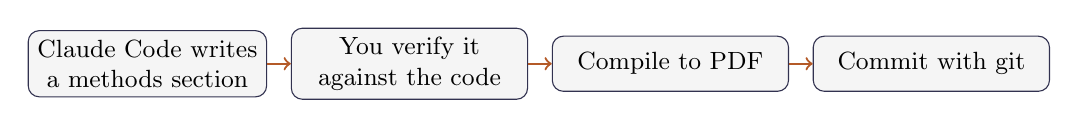
\begin{tikzpicture}[
    node distance=0.6cm and 0.3cm,
    box/.style={draw=anthropic, fill=lightgray, rounded corners, minimum width=3cm, minimum height=0.7cm, align=center, font=\small},
    arr/.style={->, thick, color=accent}
  ]
    \node[box] (write) {Claude Code writes\\a methods section};
    \node[box, right=of write] (check) {You verify it\\against the code};
    \node[box, right=of check] (compile) {Compile to PDF};
    \node[box, right=of compile] (commit) {Commit with git};

    \draw[arr] (write) -- (check);
    \draw[arr] (check) -- (compile);
    \draw[arr] (compile) -- (commit);
  \end{tikzpicture}

  \vspace{1.5em}
  {\large Everything happens in VS Code.\\[0.3em]
  Everything is version-controlled.\\[0.3em]
  Everything is visible to Claude Code.}
\end{frame}

% ══════════════════════════════════════════════════════════════════
%  BLOCK 28: EXERCISE, RESULTS TO PAPER  [1:30-1:55]
% ══════════════════════════════════════════════════════════════════

\begin{frame}{Exercise: Results $\rightarrow$ Paper (25 min)}
  Open \texttt{my\_workspace/session\_3/results\_to\_paper} in a new VS Code window. It holds \texttt{paper.tex}, \texttt{results/regression\_results.csv}, and \texttt{scripts/render\_regression\_table.py}. Everyone starts from the same results.

  \vspace{0.4em}
  \begin{enumerate}
    \small
    \item \textbf{Git first.} \texttt{git init}, have Claude Code write a \texttt{.gitignore} for \LaTeX{} build files, then commit.
    \item \textbf{Render the table.} Have Claude Code run the render script and compile \texttt{paper.tex}. Open the CSV and the \texttt{.tex} fragment yourself and check that they agree. Commit.
    \item \textbf{Results paragraph.} Have Claude Code write it from the table. Run \texttt{git diff} and read it. Keep it (commit) or revert it (\texttt{git checkout -- .}).
    \item \textbf{Cross-check.} Next slide.
  \end{enumerate}

  \vspace{0.3em}
  \alert{\small Commit $\rightarrow$ instruct $\rightarrow$ diff $\rightarrow$ decide. You should revert at least once.}
\end{frame}

\begin{frame}[fragile]{Exercise: Cross-Check Every Number}
  In a \textbf{fresh conversation}, so the checker has not just written the paragraph:

  \begin{lstlisting}[basicstyle=\ttfamily\footnotesize]
Read paper.tex and tables/regression_table.tex.
List every number in the Results paragraph, and the
table cell each one comes from. Then list every claim
(significant, robust, larger, smaller) and say whether
the table supports it. Do not edit any file.
  \end{lstlisting}

  \vspace{0.3em}
  Then answer for yourself:
  \begin{itemize}
    \small
    \item Did the check find anything you missed when you read the diff?
    \item What can this check \emph{not} catch? (Is the table itself right? Is ``causal'' justified?)
  \end{itemize}

  \vspace{0.3em}
  \alert{\small Finish with a commit. \texttt{git log -{}-oneline} should show your history.}
\end{frame}

\begin{frame}{Results $\rightarrow$ Paper: Debrief}
  \begin{enumerate}
    \item Which sentences in the paragraph went beyond what the table supports?
    \item What did you revert, and what did git make cheap?
    \item Did the cross-check find something the diff did not, or the reverse?
  \end{enumerate}

  \vspace{0.5em}
  \begin{block}{Key takeaway}
    Claude Code can write the paragraph and check the numbers. It cannot tell you whether the table is the right one to report, or whether the sentence over-reads it. That stays with you.
  \end{block}
\end{frame}

% ══════════════════════════════════════════════════════════════════
%  BLOCK 29: WHEN IT GOES WRONG  [1:55-2:01]
% ══════════════════════════════════════════════════════════════════

\begin{frame}{When It Goes Wrong: Four Failure Patterns}
  \small
  \renewcommand{\arraystretch}{1.25}
  \begin{tabular}{@{}L{0.2\textwidth}L{0.35\textwidth}L{0.38\textwidth}@{}}
    \toprule
    \textbf{Pattern} & \textbf{What you see} & \textbf{First response} \\
    \midrule
    Looping & The same fix, tried again with small variations; the error does not change & Stop it. Ask what it has tried and why each attempt failed. Change the approach, not the wording \\
    Confidently wrong & It reports success; the numbers or the code are wrong & Check against something it did not produce: an independent calculation, a test written first, a traced sample \\
    Scope creep & It edits files or changes things you did not ask about & \texttt{git diff}, revert the extras, restate the boundary in the prompt or in \texttt{CLAUDE.md} \\
    Coherence loss & Late in a long conversation it contradicts earlier decisions or drops conventions & Write the decisions to a file, start a new conversation, reload the file \\
    \bottomrule
  \end{tabular}
\end{frame}

\begin{frame}{Correct, Restart, or Do It Yourself?}
  \begin{columns}[T]
    \begin{column}{0.32\textwidth}
      \textbf{Correct it}\\[0.3em]
      {\small
      The problem is local: one wrong line, one missed instruction, and the conversation is otherwise clean.\\[0.3em]
      Say exactly what is wrong and what you expected.}
    \end{column}
    \begin{column}{0.32\textwidth}
      \textbf{Restart}\\[0.3em]
      {\small
      Two corrections have not worked, the conversation is full of failed attempts, or earlier decisions are lost.\\[0.3em]
      Commit first. Carry over only what is written in files.}
    \end{column}
    \begin{column}{0.32\textwidth}
      \textbf{Do it yourself}\\[0.3em]
      {\small
      The task is a judgment call that is yours (specification, interpretation), or you are spending longer prompting than writing.}
    \end{column}
  \end{columns}

  \vspace{0.8em}
  \begin{block}{What makes every option cheap}
    A recent commit. Reverting, restarting, and taking over by hand all start from a state you can return to.
  \end{block}
\end{frame}

% ══════════════════════════════════════════════════════════════════
%  CLOSE  [2:01]
% ══════════════════════════════════════════════════════════════════

\begin{frame}{Next Session}
  \textbf{Session 4: Power Use --- Search, Swarms, Connected Tools, Skills}

  \vspace{1em}
  \begin{itemize}
    \item Web search and literature scans, and why you check every citation
    \item Subagents: fan out work, use one as a verifier, and run a referee on a paper
    \item Connecting tools (MCP) and building a skill
  \end{itemize}

  \vspace{1em}
  \textbf{Before next session:}
  \begin{itemize}
    \item \alert{Install Node.js (LTS)} from \texttt{nodejs.org}. Check \texttt{node --version} and \texttt{npm --version}. Session 4 installs the \texttt{claude-ignore} hook with \texttt{npm}.
    \item Make git a habit on one real project: commit before every Claude Code instruction
    \item Think of a topic in your field you could run a literature search on
  \end{itemize}
\end{frame}

\begin{frame}
  ~
\end{frame}

% ══════════════════════════════════════════════════════════════════
%  BACK MATTER (after \appendix: not counted in the footer page total)
% ══════════════════════════════════════════════════════════════════

\appendix

\begin{frame}[label=backmatter]{Back Matter}
  \small
  \begin{tabular}{@{}lr@{}}
    \toprule
    \textbf{Block} & \textbf{Min} \\
    \midrule
    \hyperlink{latexbasics}{A. \LaTeX{} basics for newcomers} & 5 \\
    \hyperlink{github}{B. GitHub: vocabulary, branches, PRs, merge conflicts} & 15--20 \\
    \hyperlink{gitextras}{C. Git extras and the standalone git practice exercise} & 10--20 \\
    \hyperlink{collab}{D. \textit{Reference only:} GitHub collaboration exercise (``Your Chapter'')} & --- \\
    \hyperlink{gitpull}{E. If \texttt{git pull} fights back} & 2 \\
    \bottomrule
  \end{tabular}
\end{frame}

\begin{frame}[fragile,label=latexbasics]{\LaTeX{} Basics (For Those New to It)}
  \begin{lstlisting}[basicstyle=\ttfamily\footnotesize]
\documentclass{article}
\usepackage{booktabs}
\title{My Research Paper}
\author{Your Name}
\begin{document}
\maketitle
\section{Data Description}
We use a survey of 2,044 Polish adults...
\section{Results}
\input{output/robustness_table.tex}
\end{document}
  \end{lstlisting}

  \vspace{0.3em}
  \textbf{Key idea:} \texttt{\textbackslash input\{output/robustness\_table.tex\}} pulls in the table from Session 2. When the table updates, the paper updates.

  \vfill
  \hyperlink{backmatter}{\beamerreturnbutton{Back matter}}
\end{frame}

\begin{frame}[label=github]{What Are Git and GitHub?}
  \small
  \begin{columns}
    \column{0.7\textwidth}
    \textbf{Git} is a tool that tracks every change to every file in a project.\\
    It runs on your computer. It is free and open source.

    \vspace{0.2em}
    Think of it as ``track changes'' for your entire project directory --- not just one document, but every file: code, data descriptions, \LaTeX{} files, everything.

    \vspace{0.2em}
    \textbf{GitHub} is a website that hosts git projects online.
    \begin{itemize}
      \item It is where open-source code, replication packages, and increasingly papers live
      \item Git works entirely on your machine. GitHub is optional --- it adds backup, sharing, and collaboration
      \item This course uses git locally only. This block is for when you start sharing.
    \end{itemize}

    \vspace{0.15em}
    \begin{block}{The Key Idea}
      Git lets you save snapshots of your project at any point. You can always see what changed between snapshots, and go back to any previous one.
    \end{block}

    \column{0.25\textwidth}
    \centering
    
\includegraphics[width=0.4\columnwidth]{img/github.png}
  \end{columns}
\end{frame}

\begin{frame}{First: What Is GitHub?}
  \begin{columns}[T]
    \column{0.66\textwidth}
    \textbf{GitHub is where code lives on the internet.}

    \vspace{0.4em}
    Every project is a \emph{repository} --- a folder with all its files plus the full history of every change.

    \vspace{0.6em}
    \textbf{Two copies of everything:}
    \begin{itemize}
      \item \textbf{Remote} --- the shared version on \texttt{github.com}
      \item \textbf{Local} --- the version on your machine
    \end{itemize}

    \column{0.30\textwidth}
    \centering
    \vspace{1em}
    
\includegraphics[width=0.7\textwidth]{img/github.png}
  \end{columns}

  \vspace{0.8em}
  \begin{block}{The short version}
    GitHub hosts the \emph{shared} copy. You work on your \emph{local} copy. Git keeps them in sync.
  \end{block}
\end{frame}

\begin{frame}{The Vocabulary}
  \textbf{Five words that will keep coming back today:}

  \vspace{0.6em}
  \begin{itemize}
    \item \textbf{\texttt{clone}} --- make your first local copy of a remote repo
    \item \textbf{\texttt{pull}} --- fetch the latest changes \emph{from} the remote into your local copy
    \item \textbf{\texttt{push}} --- send your local changes \emph{to} the remote
    \item \textbf{branch} --- a parallel line of work inside the repo; changes on a branch don't affect anyone else until it's merged
    \item \textbf{pull request (PR)} --- a proposal to merge one branch into another, with a page on GitHub for review and discussion
  \end{itemize}

  \vspace{0.5em}
  \begin{block}{The flow}
    \texttt{clone} once. \texttt{pull} before you start. Make a \textbf{branch}, commit, \texttt{push}, open a \textbf{PR}. Someone reviews and merges.
  \end{block}
\end{frame}

\begin{frame}{The Course Repo}
  \textbf{Our materials live in one GitHub repo.} Everything I push goes there; everything you pull comes from there.

  \vspace{0.6em}
  \textbf{Let's look at the page together.} Things to notice:
  \begin{itemize}
    \item The \textbf{file tree} --- \texttt{session\_1/}, \texttt{session\_2/}, \ldots, \texttt{session\_4/}
    \item The \textbf{README} --- what the repo is and how to use it
    \item The \textbf{commit history} --- every change I've made, with a message
    \item The \textbf{branches} --- \texttt{main} is the shared one; others are work-in-progress
  \end{itemize}

  \vspace{0.6em}
  \begin{alertblock}{Why this matters for what's next}
    Pull conflicts happen when two people edit files in the \emph{same} repo. To see why, we need the picture of where things live.
  \end{alertblock}
\end{frame}

\begin{frame}{The Problem We Had}
  \textbf{In earlier runs of this course, someone hit a merge conflict in almost every session.}

  \vspace{0.6em}
  What we did about it:
  \begin{itemize}
    \item Deleted the local repo and recloned
    \item Asked Claude Code to resolve the conflict markers
    \item Copied work to the Desktop, wiped the directory, copied back
  \end{itemize}

  \vspace{0.8em}
  \textbf{That worked.} Everyone got unstuck. But it was a symptom fix.

  \vspace{0.8em}
  \begin{alertblock}{The Root Cause}
    You were editing files \emph{inside} the shared course repository. Every time I pushed new material, git had to reconcile your changes with mine. Conflicts were guaranteed by the structure, not by accident.
  \end{alertblock}
\end{frame}

\begin{frame}[fragile]{How GitHub Works as a Collaborator}
  \textbf{Today's git loop is the solo loop:}

  \vspace{0.3em}
  \begin{center}
  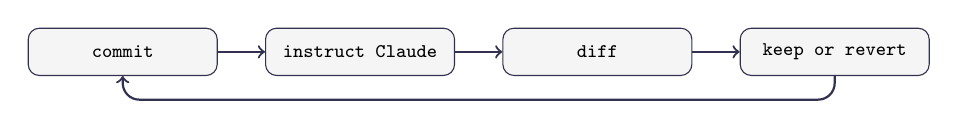
\begin{tikzpicture}[
    node distance=0.55cm and 0.6cm,
    box/.style={draw=anthropic, fill=lightgray, rounded corners, minimum width=2.4cm, minimum height=0.6cm, align=center, font=\scriptsize\ttfamily},
    arr/.style={->, thick, color=anthropic}
  ]
    \node[box] (commit) {commit};
    \node[box, right=of commit] (instruct) {instruct Claude};
    \node[box, right=of instruct] (diff) {diff};
    \node[box, right=of diff] (decide) {keep or revert};
    \draw[arr] (commit) -- (instruct);
    \draw[arr] (instruct) -- (diff);
    \draw[arr] (diff) -- (decide);
    \draw[arr, rounded corners=6pt] (decide.south) -- ++(0,-0.3) -| (commit.south);
  \end{tikzpicture}
  \end{center}

  \vspace{0.3em}
  \textbf{One person, one copy.} Everything happens on your machine.

  \vspace{0.8em}
  \textbf{Add a coauthor and two new problems appear:}
  \begin{enumerate}
    \item \textbf{Parallel work.} You both want to edit at once. Whose version wins?
    \item \textbf{Combining work.} Your changes live on your laptop, theirs on theirs. How do they become one shared version?
  \end{enumerate}

  \vspace{0.8em}
  \centering
  \alert{GitHub's answer uses two moves: branches and pull requests.}
\end{frame}

\begin{frame}[fragile]{GitHub's Answer: Branches + PRs}
  \begin{center}
  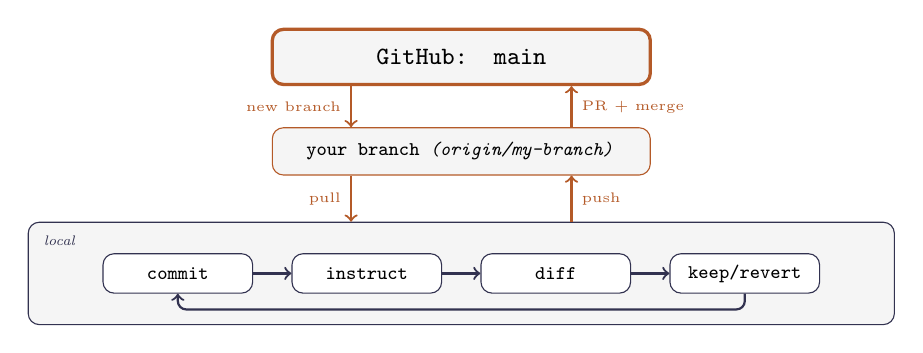
\begin{tikzpicture}[
    mainnode/.style={draw=accent, very thick, fill=lightgray, rounded corners, minimum width=4.8cm, minimum height=0.7cm, align=center, font=\small\bfseries\ttfamily},
    branchnode/.style={draw=accent, fill=lightgray, rounded corners, minimum width=4.8cm, minimum height=0.6cm, align=center, font=\scriptsize\ttfamily},
    localnode/.style={draw=anthropic, fill=lightgray, rounded corners, minimum width=11cm, minimum height=1.3cm, align=center},
    box/.style={draw=anthropic, fill=white, rounded corners, minimum width=1.9cm, minimum height=0.5cm, align=center, font=\scriptsize\ttfamily},
    arr/.style={->, thick, color=anthropic},
    arrgh/.style={->, thick, color=accent}
  ]
    \node[mainnode] (main) at (0,3.1) {GitHub: \texttt{main}};
    \node[branchnode] (branch) at (0,1.9) {your branch \textit{(origin/my-branch)}};
    \node[localnode] (local) at (0,0.35) {};

    \node[box] (c) at (-3.6, 0.35) {commit};
    \node[box] (i) at (-1.2, 0.35) {instruct};
    \node[box] (d) at (1.2, 0.35) {diff};
    \node[box] (k) at (3.6, 0.35) {keep/revert};
    \draw[arr] (c) -- (i);
    \draw[arr] (i) -- (d);
    \draw[arr] (d) -- (k);
    \draw[arr, rounded corners=3pt] (k.south) -- ++(0,-0.2) -| (c.south);

    \node[font=\tiny\itshape, text=anthropic, anchor=north west] at ([xshift=0.08cm, yshift=-0.05cm]local.north west) {local};

    \draw[arrgh] ([xshift=-1.4cm]main.south) -- ([xshift=-1.4cm]branch.north) node[midway, left, font=\tiny] {new branch};
    \draw[arrgh] ([xshift=1.4cm]branch.north) -- ([xshift=1.4cm]main.south) node[midway, right, font=\tiny] {PR + merge};
    \draw[arrgh] ([xshift=-1.4cm]branch.south) -- ([xshift=-1.4cm]local.north) node[midway, left, font=\tiny] {pull};
    \draw[arrgh] ([xshift=1.4cm]local.north) -- ([xshift=1.4cm]branch.south) node[midway, right, font=\tiny] {push};
  \end{tikzpicture}
  \end{center}

  \vspace{0.3em}
  \begin{itemize}\small
    \item \textbf{\texttt{main}} is the shared source of truth. Changes only return via PR + merge.
    \item \textbf{Your branch} is a parallel lane on GitHub --- your work stays separate until reviewed.
    \item \textbf{Locally} is where the solo loop runs, on the files of your checked-out branch.
  \end{itemize}
\end{frame}

\begin{frame}[fragile]{Working With Branches: The Commands}
  \textbf{The whole branch workflow in five moves:}
  \begin{lstlisting}[basicstyle=\ttfamily\scriptsize]
# 1. Start from an up-to-date main
git checkout main
git pull
# 2. Create a new branch
git branch my-branch-name
# 3. Switch to it
git checkout my-branch-name
# 4. Commit
git add <files>
git commit -m "..."
# 5. Push (first time uses -u; later pushes: git push)
git push -u origin my-branch-name
  \end{lstlisting}

  \alert{\small \texttt{git branch} lists branches (\texttt{*} marks current). Commit before switching --- uncommitted edits follow you between branches.}
\end{frame}

\begin{frame}[fragile]{What Is a Pull Request?}
  \textbf{A pull request (PR) is the proposal to merge one branch into another.} Everyone branches off \texttt{main}, works independently, then opens a PR to rejoin.

  \vspace{0.3em}
  \begin{center}
  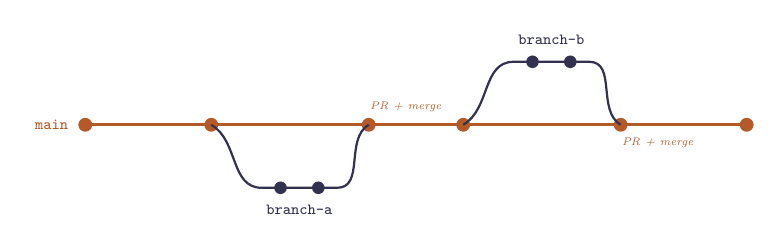
\begin{tikzpicture}[
    scale=0.8, transform shape,
    mcommit/.style={circle, fill=accent, minimum size=0.22cm, inner sep=0},
    bcommit/.style={circle, fill=anthropic, minimum size=0.2cm, inner sep=0},
    mainline/.style={very thick, color=accent},
    branchline/.style={thick, color=anthropic},
    lbl/.style={font=\scriptsize\ttfamily},
    mlbl/.style={font=\tiny\itshape, text=accent}
  ]
    \foreach \x in {0, 2, 4.5, 6, 8.5, 10.5} {
      \node[mcommit] at (\x, 0) {};
    }
    \draw[mainline] (0,0) -- (10.5,0);
    \node[lbl, text=accent, anchor=east] at (-0.15, 0) {\textbf{main}};

    \draw[branchline] (2,0) to[out=-30, in=180] (2.8,-1) -- (4,-1) to[out=0, in=210] (4.5, 0);
    \node[bcommit] at (3.1, -1) {};
    \node[bcommit] at (3.7, -1) {};
    \node[lbl, text=anthropic, anchor=north] at (3.4, -1.15) {branch-a};
    \node[mlbl, anchor=south west] at (4.4, 0.08) {PR + merge};

    \draw[branchline] (6,0) to[out=30, in=180] (6.8,1) -- (8,1) to[out=0, in=150] (8.5, 0);
    \node[bcommit] at (7.1, 1) {};
    \node[bcommit] at (7.7, 1) {};
    \node[lbl, text=anthropic, anchor=south] at (7.4, 1.15) {branch-b};
    \node[mlbl, anchor=north west] at (8.4, -0.08) {PR + merge};
  \end{tikzpicture}
  \end{center}

  \vspace{0.2em}
  \textbf{On the PR page:} a diff, a conversation thread, and an approve-and-merge button gated by the drafter's assigned \textbf{reviewer}.

  \vspace{0.3em}
  \alert{\small On a collaborative repo, every PR has an assigned reviewer. They have to click approve \emph{and} merge --- nothing reaches \texttt{main} until they do.}
\end{frame}

\begin{frame}[fragile]{Push vs.\ Pull Request: Two Different Moves}
  \textbf{These get conflated constantly, but they do different jobs.}

  \vspace{0.5em}
  \begin{columns}[T]
    \column{0.48\textwidth}
    \textbf{\texttt{git push}}
    \begin{itemize}\small
      \item Uploads your local commits to \emph{your branch} on GitHub
      \item Pure sync --- mechanical, instant, no review
      \item Touches only your branch; \texttt{main} is untouched
      \item You do it \emph{many} times as you work
    \end{itemize}

    \column{0.48\textwidth}
    \textbf{Pull request (PR)}
    \begin{itemize}\small
      \item Proposes merging your branch \emph{into} \texttt{main}
      \item A request --- reviewed, discussed, then merged
      \item The \emph{merge} is what actually changes \texttt{main}
      \item One per chunk of work; push again and it updates
    \end{itemize}
  \end{columns}

  \vspace{0.6em}
  \begin{block}{The one-liner}
    \textbf{Push} sends your commits to your branch. \textbf{A PR} asks to fold that branch into \texttt{main}. Push moves code \emph{to the server}; only a \emph{merged} PR moves it \emph{into the shared version}.
  \end{block}

  \vspace{0.2em}
  \alert{\small You can push a hundred times and \texttt{main} never changes --- it changes only when a PR is merged.}
\end{frame}

\begin{frame}[fragile,label=troubleshooting]{Troubleshooting: When GitHub Fights Back}
  \textbf{Common failure modes during the exercise --- and the fix.}

  \vspace{0.2em}
  \begin{itemize}\footnotesize
    \item \textbf{Authentication fails on first push.} Run \texttt{gh auth login} and pick HTTPS + browser. (\texttt{brew install gh} first if needed.)

    \item \textbf{``Updates were rejected''} --- \texttt{main} moved while you worked. \\
    \texttt{git pull -{}-rebase origin main \&\& git push}

    \item \textbf{Conflict markers (\texttt{<<<<<<<}) in a file.} Open it, edit to the version you want, delete the markers. Then \texttt{git add <file>} and \texttt{git rebase -{}-continue} (or \texttt{git commit} if merging). \hyperlink{merge-conflicts}{\alert{Walkthrough $\rightarrow$}}

    \item \textbf{You committed to \texttt{main} by accident.} Save the work to a new branch, then rewind \texttt{main}:
    \begin{lstlisting}[basicstyle=\ttfamily\scriptsize]
git checkout -b chapter-N
git checkout main && git reset --hard origin/main
git checkout chapter-N
    \end{lstlisting}

    \item \textbf{PR opened against the wrong base.} Edit the base branch in the GitHub UI at the top of the PR --- no need to close and reopen.

    \item \textbf{Stuck for more than 90 seconds.} Flag me. Don't silently spin --- the fix is usually one command.
  \end{itemize}
\end{frame}

\begin{frame}[fragile,label=merge-conflicts]{Anatomy of a Merge Conflict}
  \textbf{When git can't auto-combine two versions of the same lines, it leaves the file marked up like this:}

  \vspace{0.3em}
  \begin{lstlisting}[basicstyle=\ttfamily\footnotesize]
The keynote speaker took the stage.
<<<<<<< HEAD
He launched into a 90-minute monologue about LLMs.
=======
She fumbled with the slide remote for two full minutes.
>>>>>>> origin/main
The audience applauded politely.
  \end{lstlisting}

  \vspace{0.3em}
  \textbf{Three parts:}
  \begin{itemize}\footnotesize
    \item \texttt{<<<<<<< HEAD} --- start of \textbf{your} version (the branch you're on)
    \item \texttt{=======} --- divider
    \item \texttt{>>>>>>> origin/main} --- end, plus the name of the \textbf{incoming} version
  \end{itemize}

  \vspace{0.2em}
  \alert{Git isn't broken. It just can't tell which version you want --- and is asking you to decide.}
\end{frame}

\begin{frame}[fragile]{Resolving a Conflict by Hand}
  \textbf{1. Find them:} \texttt{\small git status} \;\;\textit{\small (conflicted files appear under ``both modified'')}

  \vspace{0.4em}
  \textbf{2. Open each one. Edit until only the version you want remains --- no markers.}

  \vspace{0.2em}
  \begin{columns}[T]
    \column{0.48\textwidth}
    \textit{\small Before:}
    \begin{lstlisting}[basicstyle=\ttfamily\scriptsize]
<<<<<<< HEAD
He launched into a 90-min
monologue about LLMs.
=======
She fumbled with the slide
remote for two full minutes.
>>>>>>> origin/main
    \end{lstlisting}

    \column{0.48\textwidth}
    \textit{\small After (keep one, the other, or merge):}
    \begin{lstlisting}[basicstyle=\ttfamily\scriptsize]
She fumbled with the slide
remote for two full minutes,
then launched into a 90-min
monologue about LLMs.
    \end{lstlisting}
  \end{columns}

  \vspace{0.3em}
  \textbf{3. Stage the file and continue.}
  \begin{lstlisting}[basicstyle=\ttfamily\scriptsize]
git add chapters/chapter_3.md && git rebase --continue
# (or: git commit, if you were merging instead of rebasing)
  \end{lstlisting}

  {\footnotesize \textbf{Want to bail out?} \texttt{git rebase -{}-abort} (or \texttt{git merge -{}-abort}) reverts to the pre-conflict state.}
\end{frame}

\begin{frame}[fragile]{Letting Claude Resolve It}
  \textbf{Claude Code is good at the mechanical part --- finding the markers and proposing a sensible merge.}

  \vspace{0.3em}
  A prompt that works:
  \begin{lstlisting}[basicstyle=\ttfamily\footnotesize]
There's a merge conflict in chapters/chapter_3.md.
Read both sides, propose a resolution that keeps the
intent of both, and apply it. Show me the diff first
- do not commit.
  \end{lstlisting}

  \vspace{0.4em}
  \begin{columns}[T]
    \column{0.48\textwidth}
    \textbf{Safe to delegate:}
    \begin{itemize}\footnotesize
      \item Trivial conflicts (formatting, adjacent edits)
      \item One side is clearly the newer or correct version
      \item Prose where the diff is short and you can read it end-to-end
    \end{itemize}

    \column{0.48\textwidth}
    \textbf{Do it yourself:}
    \begin{itemize}\footnotesize
      \item Code where behavior changes --- you need to understand both sides
      \item Numerical results, tables, anything you'd want to verify line-by-line
      \item Conflicts touching more than a handful of files
    \end{itemize}
  \end{columns}

  \vspace{0.4em}
  \alert{\small Always read the diff. ``Resolved'' is not the same as ``correct.''}
  \vfill
  \hfill \hyperlink{backmatter}{\beamerreturnbutton{Back matter}}
\end{frame}

\begin{frame}[label=gitextras]{Why Researchers Should Care About Git}
  \begin{columns}
    \column{0.7\textwidth}
    \textbf{Without git, you have probably done this:}
    \begin{itemize}
      \item \texttt{analysis\_v2.py}, \texttt{analysis\_v2\_final.py}, \texttt{analysis\_v2\_final\_REAL.py}
      \item ``Which version of the cleaning script produced these results?''
      \item ``I changed something last week and now the code is broken''
    \end{itemize}

    \vspace{0.5em}
    \textbf{With git:}
    \begin{itemize}
      \item One file, full history. Every version is recoverable.
      \item You can see exactly what changed, when, and why.
      \item You can undo any change --- even from weeks ago.
    \end{itemize}

    \vspace{0.5em}
    Git is useful for any research project. But when you are working with an agent that modifies your files directly, it goes from useful to \alert{essential}.

    \column{0.25\textwidth}
    \vspace{-0.5cm}
    \centering
    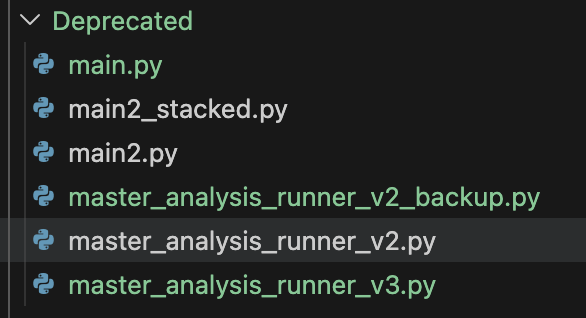
\includegraphics[width=0.85\columnwidth]{img/copies_of_copies.png}
  \end{columns}
\end{frame}

\begin{frame}{You Have Already Seen This}

  \begin{center}
    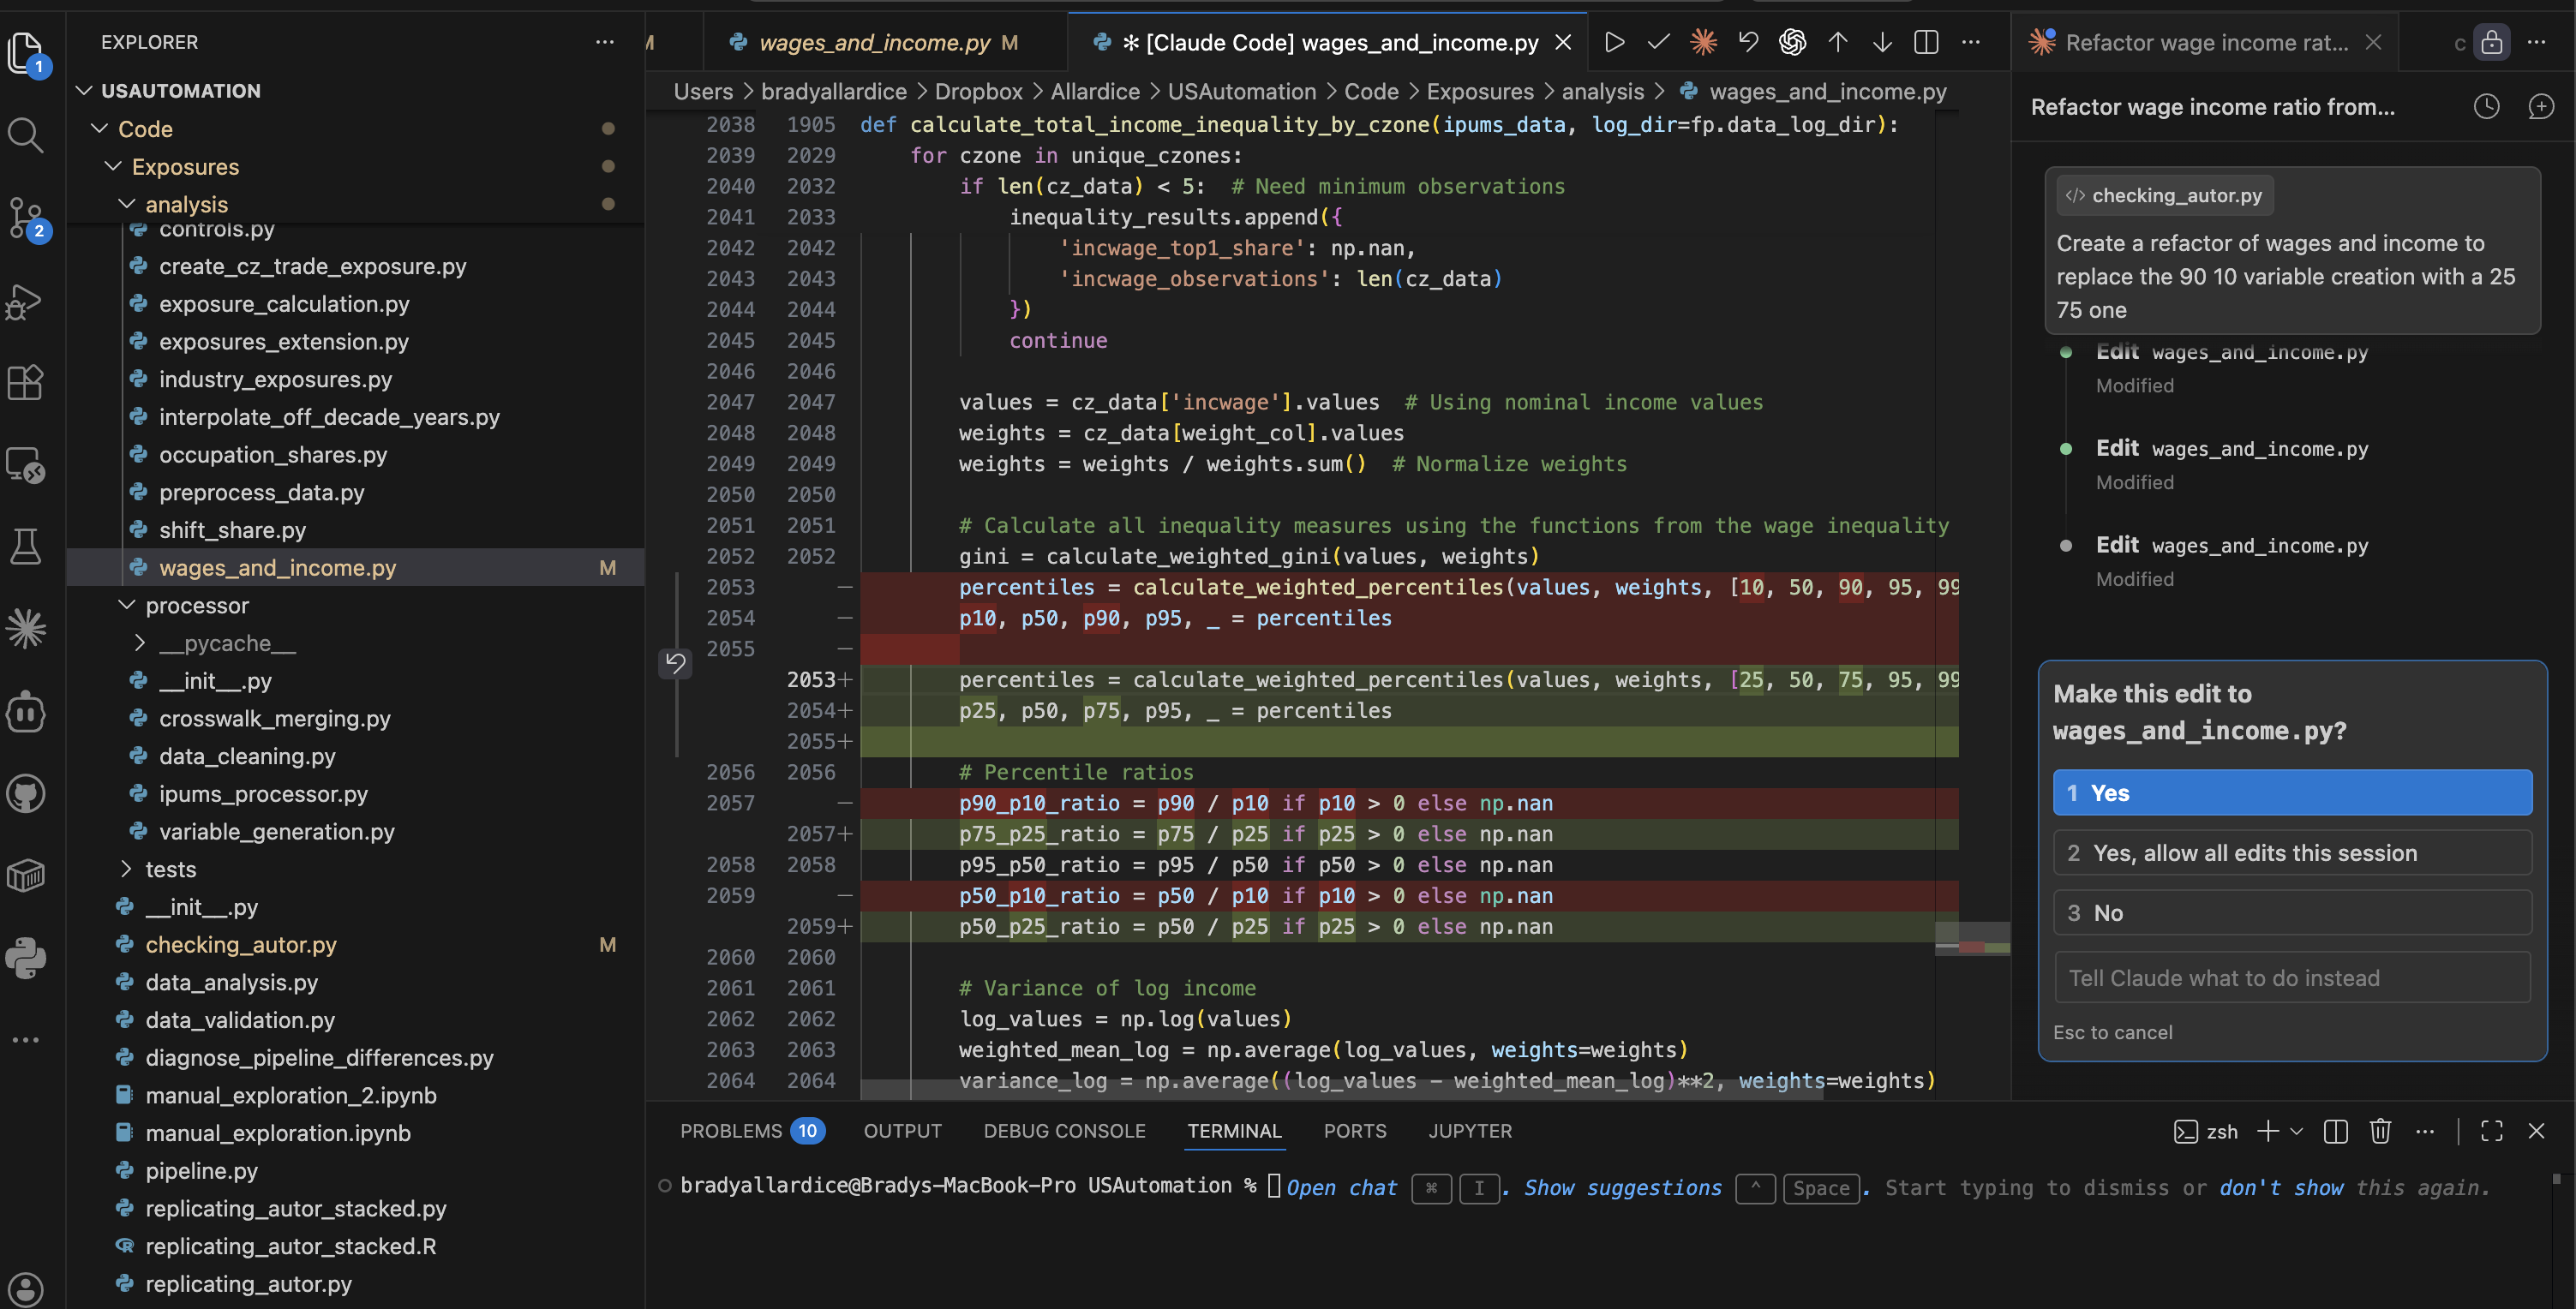
\includegraphics[width=0.70\textwidth]{img/claude_mid_update.png}
  \end{center}

  {\small Red = removed, green = added. You have been reading diffs since Session 1.\\
  \textbf{In VS Code:} When working directly in the editor, you see the \texttt{git diff} visually before you accept the change. This shows exactly what Claude Code changed.}
\end{frame}

\begin{frame}[fragile]{A Typical \texttt{.gitignore}}
  \small
  \textbf{\texttt{.gitignore}}
  \begin{lstlisting}[basicstyle=\ttfamily\tiny]
# Folders
data/raw/
data/*/administrative/
output/

# Specific files
.env
.DS_Store

# Large Data Files
data_merged.csv
copy_of_internet.csv

# Python cache (auto-generated, don't need)
__pycache__/
  \end{lstlisting}

  \vspace{0.15em}
  {\small \textbf{Wildcards:} \texttt{*} matches any characters.
  \begin{itemize}
    \item \texttt{*.pyc} = all \texttt{.pyc} files (anywhere in project)
    \item \texttt{data.*.csv} = \texttt{data.raw.csv}, \texttt{data.clean.csv}, etc.
    \item \texttt{analysis\_*.py} = \texttt{analysis\_v1.py}, \texttt{analysis\_v2.py}, etc.
  \end{itemize}
  \textbf{Folders} must end with \texttt{/} (e.g., \texttt{output/}, \texttt{\_\_pycache\_\_/})}

  \vspace{0.1em}
  {\tiny \textbf{Path scope:} \texttt{*} = any level  \textbar\  \texttt{**} = any depth  \textbar\  \texttt{data\_merged.csv} matches anywhere  \textbar\  \texttt{data/data\_merged.csv} matches only in \texttt{data/}.}
\end{frame}

\begin{frame}{So Where Does the Data Go?}
  \textbf{Why git is bad for data:}
  \begin{itemize}
    \item Git stores \textit{every version} of every file. A 200MB CSV edited 10 times = 2GB of history.
    \item Git compares files line by line. Change one cell in a CSV and git sees the entire row as new.
    \item Large files slow down every git operation --- commits, diffs, cloning.
  \end{itemize}

  \vspace{0.3em}
  \textbf{For most research projects (data under a few GB):}
  \begin{itemize}
    \item Keep data in a synced folder: \textbf{Dropbox}, \textbf{OneDrive}, \textbf{Google Drive}
    \item Your code lives in git. Your data lives next to it. Your \texttt{.gitignore} keeps them separate.
    \item Simple, familiar, and good enough for most social science workflows
  \end{itemize}

  \vspace{0.3em}
  \textbf{For larger or more complex needs:}
  \begin{itemize}
    \item \textbf{Object storage:} AWS S3, Google Cloud Storage --- cheap, scalable
    \item \textbf{Data versioning:} DVC (Data Version Control) --- git-like tracking for large files
  \end{itemize}

  \vspace{0.2em}
  {\small You do not need these today. But if your data outgrows Dropbox, they exist.}
\end{frame}

\begin{frame}{Exercise Part 1: Choose Your Project}
  \textbf{Option A: Your own research project}
  \begin{itemize}
    \item Open your project folder in VS Code: File → New Window → File → Open Folder
    \item Use whatever code and data you have in that project
  \end{itemize}

  \vspace{0.5em}
  \textbf{Option B: Practice sandbox}
  \begin{itemize}
    \item On your Desktop, create a new folder: \texttt{mkdir \textasciitilde/Desktop/session\_2\_git\_practice}
    \item Copy Session 2 materials into it: \texttt{cp -r \textasciitilde/my\_workspace/session\_2/* \textasciitilde/Desktop/session\_2\_git\_practice/}
    \item Open it in VS Code: File → New Window → File → Open Folder → select \texttt{session\_2\_git\_practice} on Desktop
  \end{itemize}

  \vspace{0.5em}
  Pick one and open it in VS Code.
\end{frame}

\begin{frame}{Exercise Part 1: Initialize and Commit (10 min)}
  Now, in your chosen project directory:

  \begin{enumerate}
    \item {\small \textbf{Create a \texttt{.gitignore}} FIRST:} In VS Code (File → New File → name it .gitignore) or terminal (\texttt{echo ".env" > .gitignore}). Ask Claude Code to help. Include \texttt{.env}, large data files, regenerated output, and system files.

    {\small \alert{Important (Option B):} You will find a \texttt{.env} file with my real credentials. Make sure it is in \texttt{.gitignore} so it is never committed.}

    \vspace{0.08em}
    \item {\small \textbf{Initialize git:}} \texttt{git init} then \texttt{git add -A \&\& git commit -m "Initial commit"}

    \vspace{0.08em}
    \item {\small \textbf{Run:}} \texttt{git log --oneline}
  \end{enumerate}
\end{frame}

\begin{frame}{Exercise Part 2: The Cycle (25 min)}
  Do this \textbf{three times} (you decide what changes):

  \vspace{0.3em}
  \begin{enumerate}
    \item \textbf{Commit} your current state
    \item \textbf{Instruct Claude Code} to make a change. Pick anything:
    \begin{itemize}
      \item Add a control variable, refactor into functions, change sample restriction
      \item Fix a bug, improve documentation, rename variables
      \item Add a new analysis, create a visualization, write a summary
    \end{itemize}
    \item \textbf{Run} \texttt{git diff} and read what changed
    \item \textbf{Decide:} keep (commit) or revert (\texttt{git checkout -- .})
  \end{enumerate}

  \vspace{0.3em}
  {\small \textbf{Goal:} Try to revert at least once. See that you can always undo.}

  {\tiny If you revert and regret it, you can recover the changes from your last commit using \texttt{git reflog} and \texttt{git checkout}.}

  \vspace{0.1em}
  \alert{Commit → Instruct → Diff → Decide}
\end{frame}

\begin{frame}{Git Debrief}
  \textbf{Discussion:}
  \begin{itemize}
    \item Did Claude Code change any files you did not expect?
    \item Was the diff easy to read? What was confusing?
    \item Did anyone revert a change? What went wrong?
  \end{itemize}

  \vspace{1em}
  \begin{block}{The Habit}
    \textbf{Commit $\rightarrow$ Instruct $\rightarrow$ Diff $\rightarrow$ Decide.}\\[0.3em]
    This is not optional when working with an agent that modifies your files. It is the minimum responsible workflow.
  \end{block}

  \vfill
  \hfill \hyperlink{backmatter}{\beamerreturnbutton{Back matter}}
\end{frame}

\begin{frame}[label=collab]{Collaboration, Live}
  \textbf{Time to see the whole loop on a real repo.} I'll walk through branches, commits, push, PR, review, and merge --- on \texttt{github.com/bradyallardice/github\_collaboration\_practice}.

  \vspace{0.8em}
  \textbf{What I'll do:} write a list of characters for a story. You pick which story:

  \vspace{0.3em}
  \begin{enumerate}
    \item \textbf{The Conference From Hell} --- every session, break, and hallway moment at an academic conference goes sideways
    \item \textbf{The Dissertation That Wrote Itself} --- a PhD student's dissertation has gained sentience; each chapter is one night of it taking new liberties
    \item \textbf{The Department Mouse} --- a very literate mouse is stealing specific things from the department; it appears to have a plan
  \end{enumerate}

  \vspace{0.6em}
  \alert{Watch the steps. Ask questions. I'll end with the cast pushed to \texttt{main}.}

  \vspace{0.4em}
  \alert{\small Reference only. This needs GitHub accounts and collaborator access set up in advance.}
\end{frame}

\begin{frame}{Before We Go Further: GitHub Access}
  \textbf{Two quick things:}

  \vspace{0.8em}
  \begin{enumerate}
    \item \textbf{If you haven't already emailed me your GitHub username, write it on the paper going around now.}

    \vspace{0.4em}
    \item \textbf{Everyone: check your email and accept the collaboration request for the class repo.} Without it you can't push a branch or open a PR.
  \end{enumerate}

  \vspace{0.8em}
  The invite appears as an email from GitHub, and also as a banner on the repo page if you're logged in. Click \textbf{Accept invitation}.

  \vspace{0.5em}
  \alert{One minute. Shout if it doesn't show up --- I'll re-send.}
\end{frame}

\begin{frame}{\ldots Now You're Going to Write the Story}
  \textbf{That repo I just pushed to? You're going to write the rest of it.}

  \vspace{0.6em}
  Each of you claims one of the 16 chapter slots, featuring the cast I just pushed. Write, branch, PR, merge your own chapter --- all the way through. At the end, we assemble every chapter and read the story out loud.

  \vspace{0.8em}
  \textbf{Your chapter should feature at least one of the named characters.} Beyond that, go wherever it takes you.

  \vspace{0.6em}
  \alert{The writing is short on purpose. The point is the Git workflow, not the prose.}
\end{frame}

\begin{frame}{Your Chapter}
  \textbf{I've assigned each of you a specific chapter.} Open \texttt{CHAPTERS.md} at the root of the class repo --- your name is next to a numbered slot. That's your chapter.

  \vspace{0.5em}
  \textbf{Then you run the whole loop yourself:}
  \begin{itemize}
    \item Branch from \texttt{main}, write your chapter at \texttt{chapters/chapter\_N.md}
    \item Commit, push, open a PR
    \item Approve and merge your own PR
  \end{itemize}

  \vspace{0.6em}
  \begin{block}{Ground rules}
    \begin{itemize}
      \item \textbf{Length doesn't matter.} A paragraph is fine.
      \item \textbf{Don't try to match other chapters.} You can't --- everyone is writing simultaneously.
      \item \textbf{Don't polish.} Five minutes. Write, push, merge, move on.
    \end{itemize}
  \end{block}
\end{frame}

\begin{frame}[fragile]{Reference Card}
  \textbf{1. Clone the repo, open it, branch, write, commit, push:}
  \begin{lstlisting}[basicstyle=\ttfamily\tiny]
git clone https://github.com/bradyallardice/github_collaboration_practice.git
cd github_collaboration_practice
code .                            # open the repo in VS Code
git checkout -b chapter-N
# write your assigned chapter at chapters/chapter_N.md
git add chapters/chapter_N.md
git commit -m "Chapter N"
git push -u origin chapter-N
  \end{lstlisting}

  \vspace{0.3em}
  \textbf{2. Open and merge the PR on GitHub:}
  \begin{enumerate}\small
    \item Click the \textbf{Compare \& pull request} banner, base = \texttt{main}
    \item \textbf{Create pull request}
    \item \textbf{Merge pull request} $\rightarrow$ \textbf{Confirm merge}
  \end{enumerate}

  \vspace{0.3em}
  \centerline{\small Something break? \hyperlink{troubleshooting}{\alert{$\rightarrow$ Troubleshooting GitHub}}}
\end{frame}

\begin{frame}{What to Expect}
  \textbf{Some of you will finish. Some will not. Both are fine.}

  \vspace{0.6em}
  The goal is that \emph{everyone sees the loop end-to-end}: branch, push, PR, merge. Even if you need help at every step, you will recognize the shape next time.

  \vspace{0.6em}
  \textbf{What will go wrong (for some of you):}
  \begin{itemize}
    \item \textbf{Push rejected} because \texttt{main} moved. Run \texttt{git pull --rebase origin main} and push again.
    \item \textbf{PR opened against the wrong base.} Edit the base branch in the GitHub UI, or close and reopen.
    \item \textbf{You get stuck for more than 90 seconds.} Flag me. Don't silently spin.
  \end{itemize}

  \vspace{0.4em}
  \alert{After all PRs are merged, I'll run the assembly script and read us the story.}
  \vfill
  \hfill \hyperlink{backmatter}{\beamerreturnbutton{Back matter}}
\end{frame}

\begin{frame}[fragile,label=gitpull]{If \texttt{git pull} Fights Back}
  If you committed work inside the repo, \texttt{git pull} will complain. Run this recovery in the course repo, then continue with Steps 2--3:

  \vspace{0.3em}
  \begin{lstlisting}[basicstyle=\ttfamily\footnotesize]
git stash -u                      # save uncommitted edits
git branch backup-prework         # save any local commits
git fetch origin
git reset --hard origin/student   # match the server
git stash pop                     # skip if stash was empty
  \end{lstlisting}

  \vspace{0.2em}
  {\small Your old commits live on \texttt{backup-prework}. If that name exists, add a suffix: \texttt{backup-prework-2}.}

  \vfill
  \hyperlink{ritual}{\beamerreturnbutton{Back to the ritual}} \hfill \hyperlink{backmatter}{\beamerreturnbutton{Back matter}}
\end{frame}

\end{document}
